\chapter{Analysis of spatial-diversity with a numerical simulator}
The previous chapter introduced the idea of exploiting spatial-diversity to provide more priority levels for flow classification. It was discussed why in principle such technique could yield flow completion time gains, especially when few priority queues are available. It was explained that adopting a spatial-diversity demotion has strong implication on the traffic load balancing, since flow routing becomes priority-dependent.  A few questions arises soon: how to choose the thresholds to distribute the load on the topology? What are the relationships between the priority granularity in 
single interfaces and spatial diversity? Is the best choice to use all spines for incremental priorities when the topology is big? The goal of this chapter is to validate these intuitive hints with numerical results and to shed the light on the benefits and the restraints of the proposed algorithm. In particular, it will go through an exhaustive analysis of the system by delivering plenty of numerical experiments obtained with a custom flow simulator implemented in Python. This simulator does not capture any of the complex dynamics inherent to a real packet network, it does not have any protocol stack implemented neither at traffic sources modules nor in the switching modules. Rather, it is a job-oriented queueing simulator that does not care about packets but only runs flow arrivals and serve them in queuing modules. Its purpose is to provide a clean baseline numerical analysis not plagued by possible side effects due to network misconfiguration.
\section{Spatial-diversity framework}

\subsection{Problem abstraction}
To tackle spatial-diversity in the initial phase and get a first glance about its effectiveness, three queuing systems are compared. They are shown in Fig.\ref{fig:three-system-comparison}. 

\begin{figure}
	\centering
	\begin{subfigure}[b]{0.3\textwidth}
		\centering
		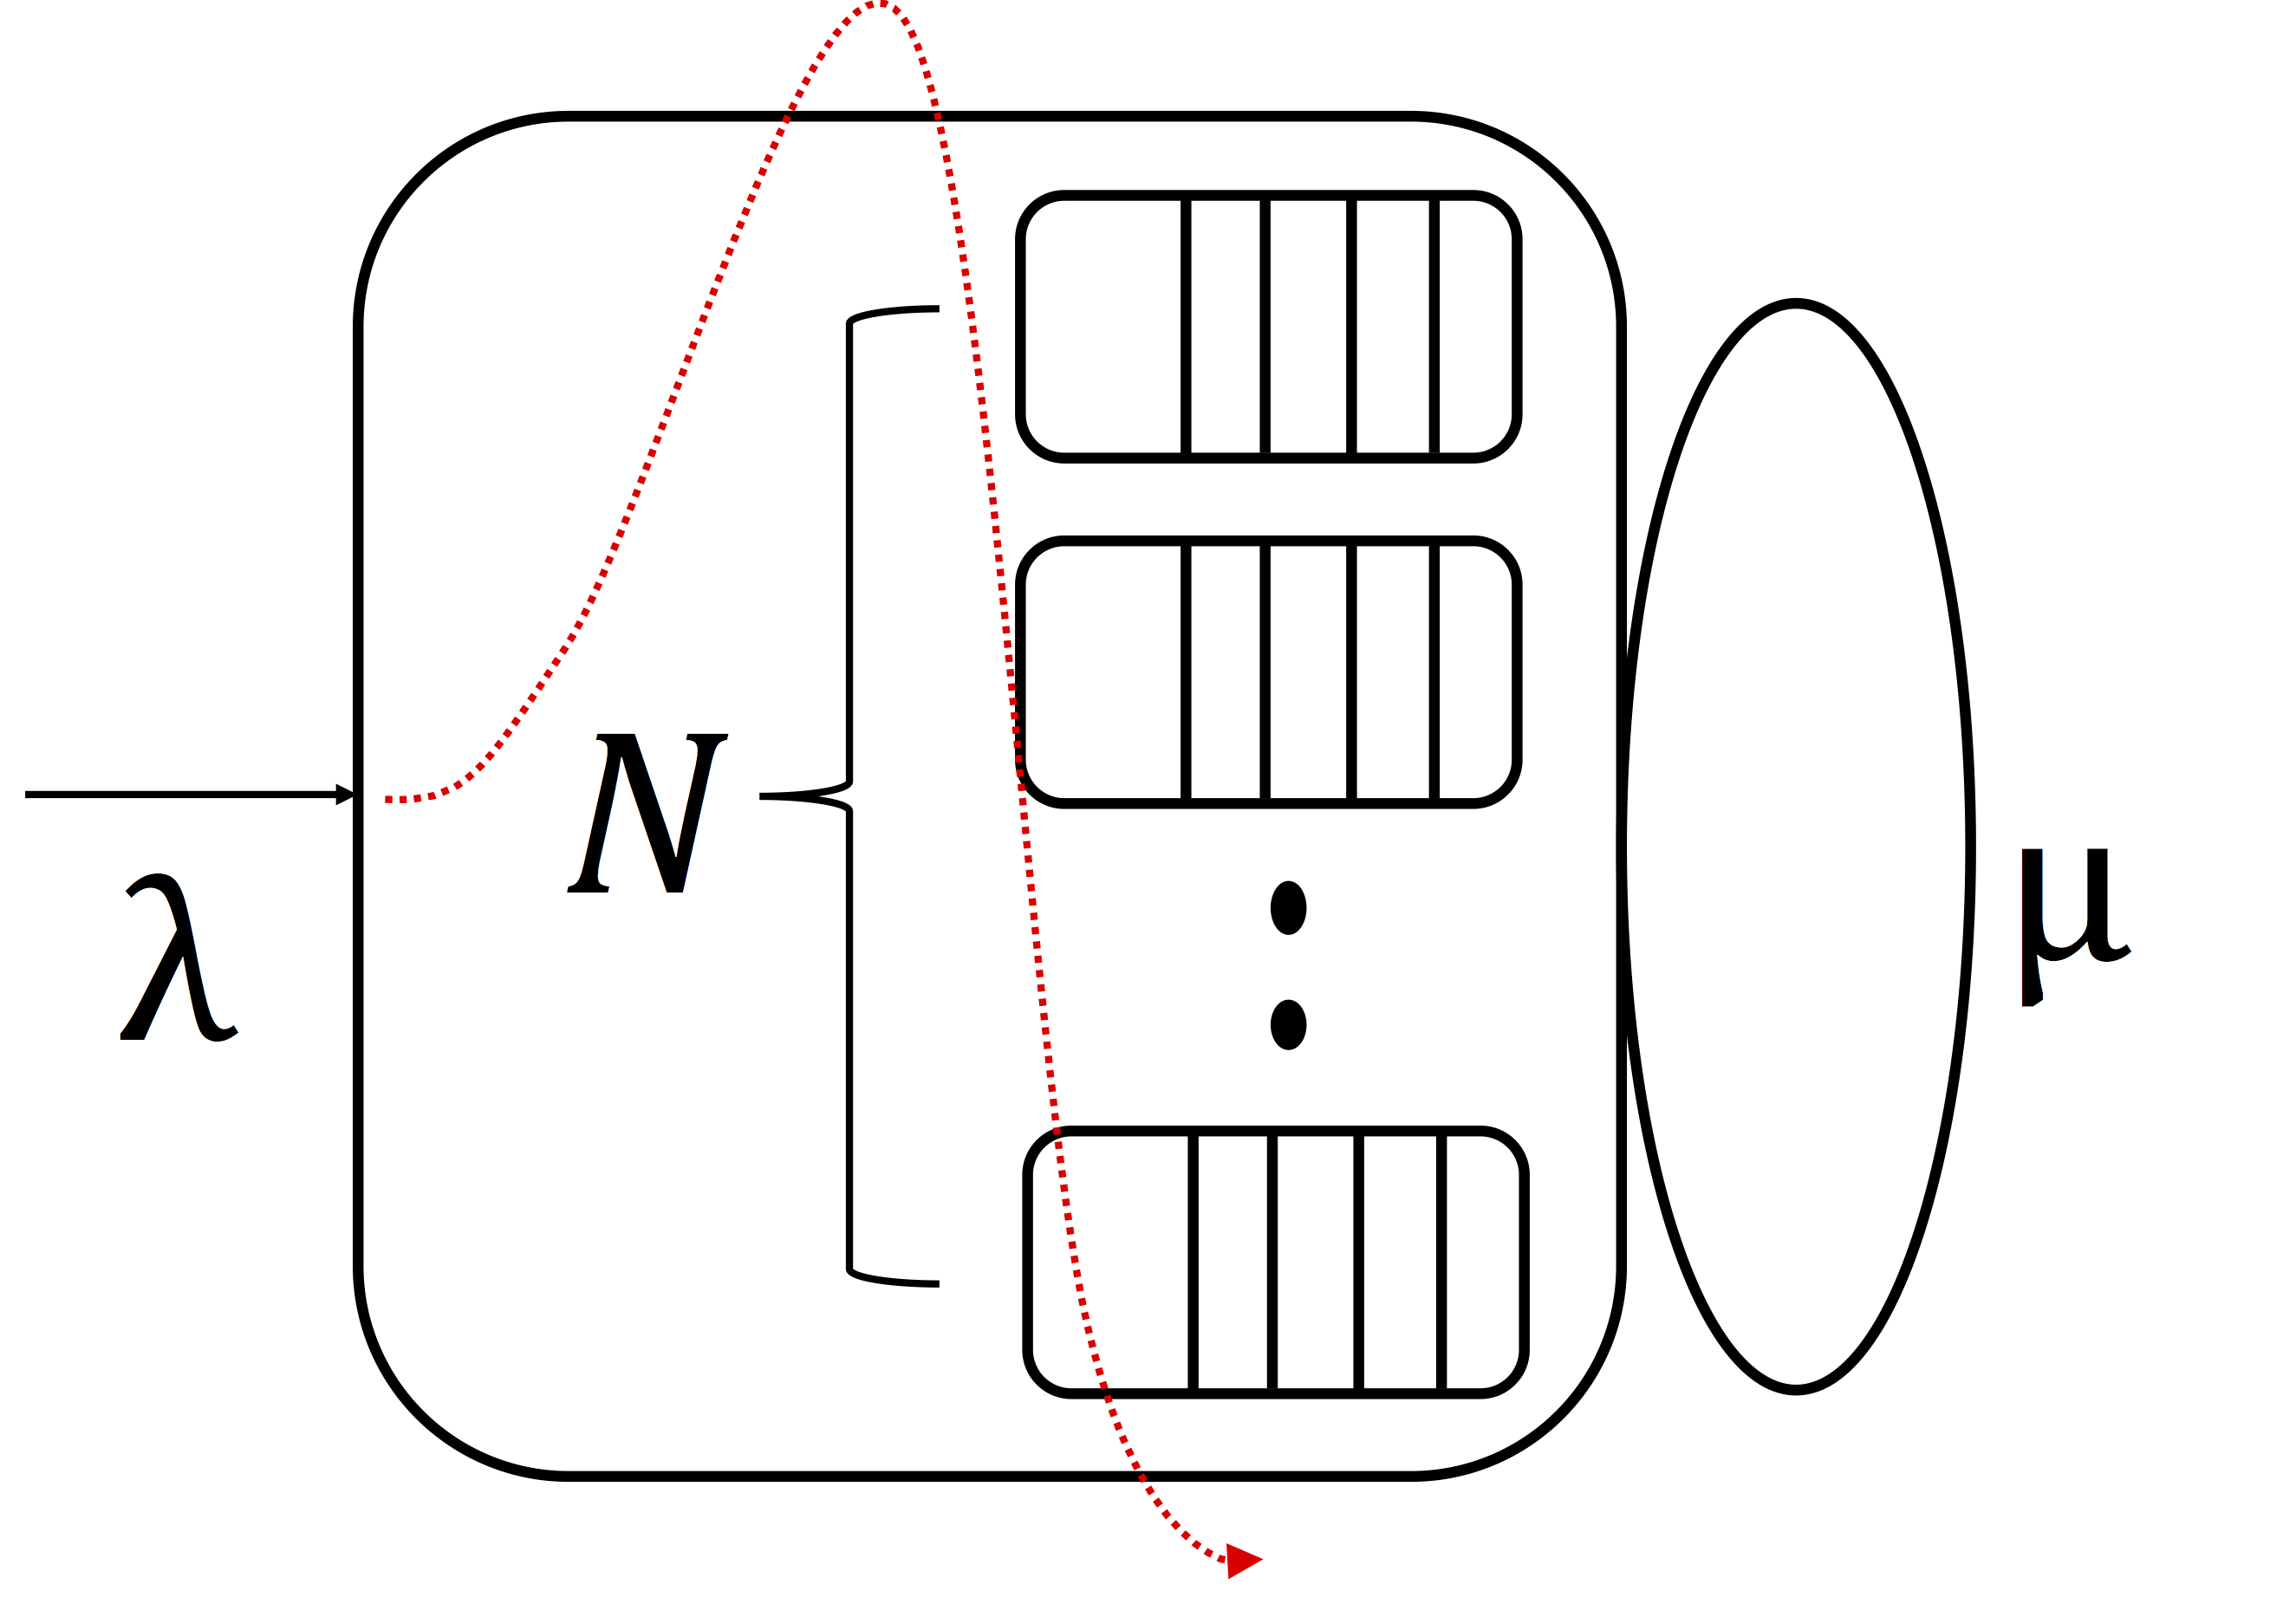
\includegraphics[width=\textwidth]{Chapter3/Figures/switchone}
		\smallskip
		\caption{Super-Server}
		\label{fig:switchone}
	\end{subfigure}
	\hfill
	\begin{subfigure}[b]{0.3\textwidth}
		\centering
		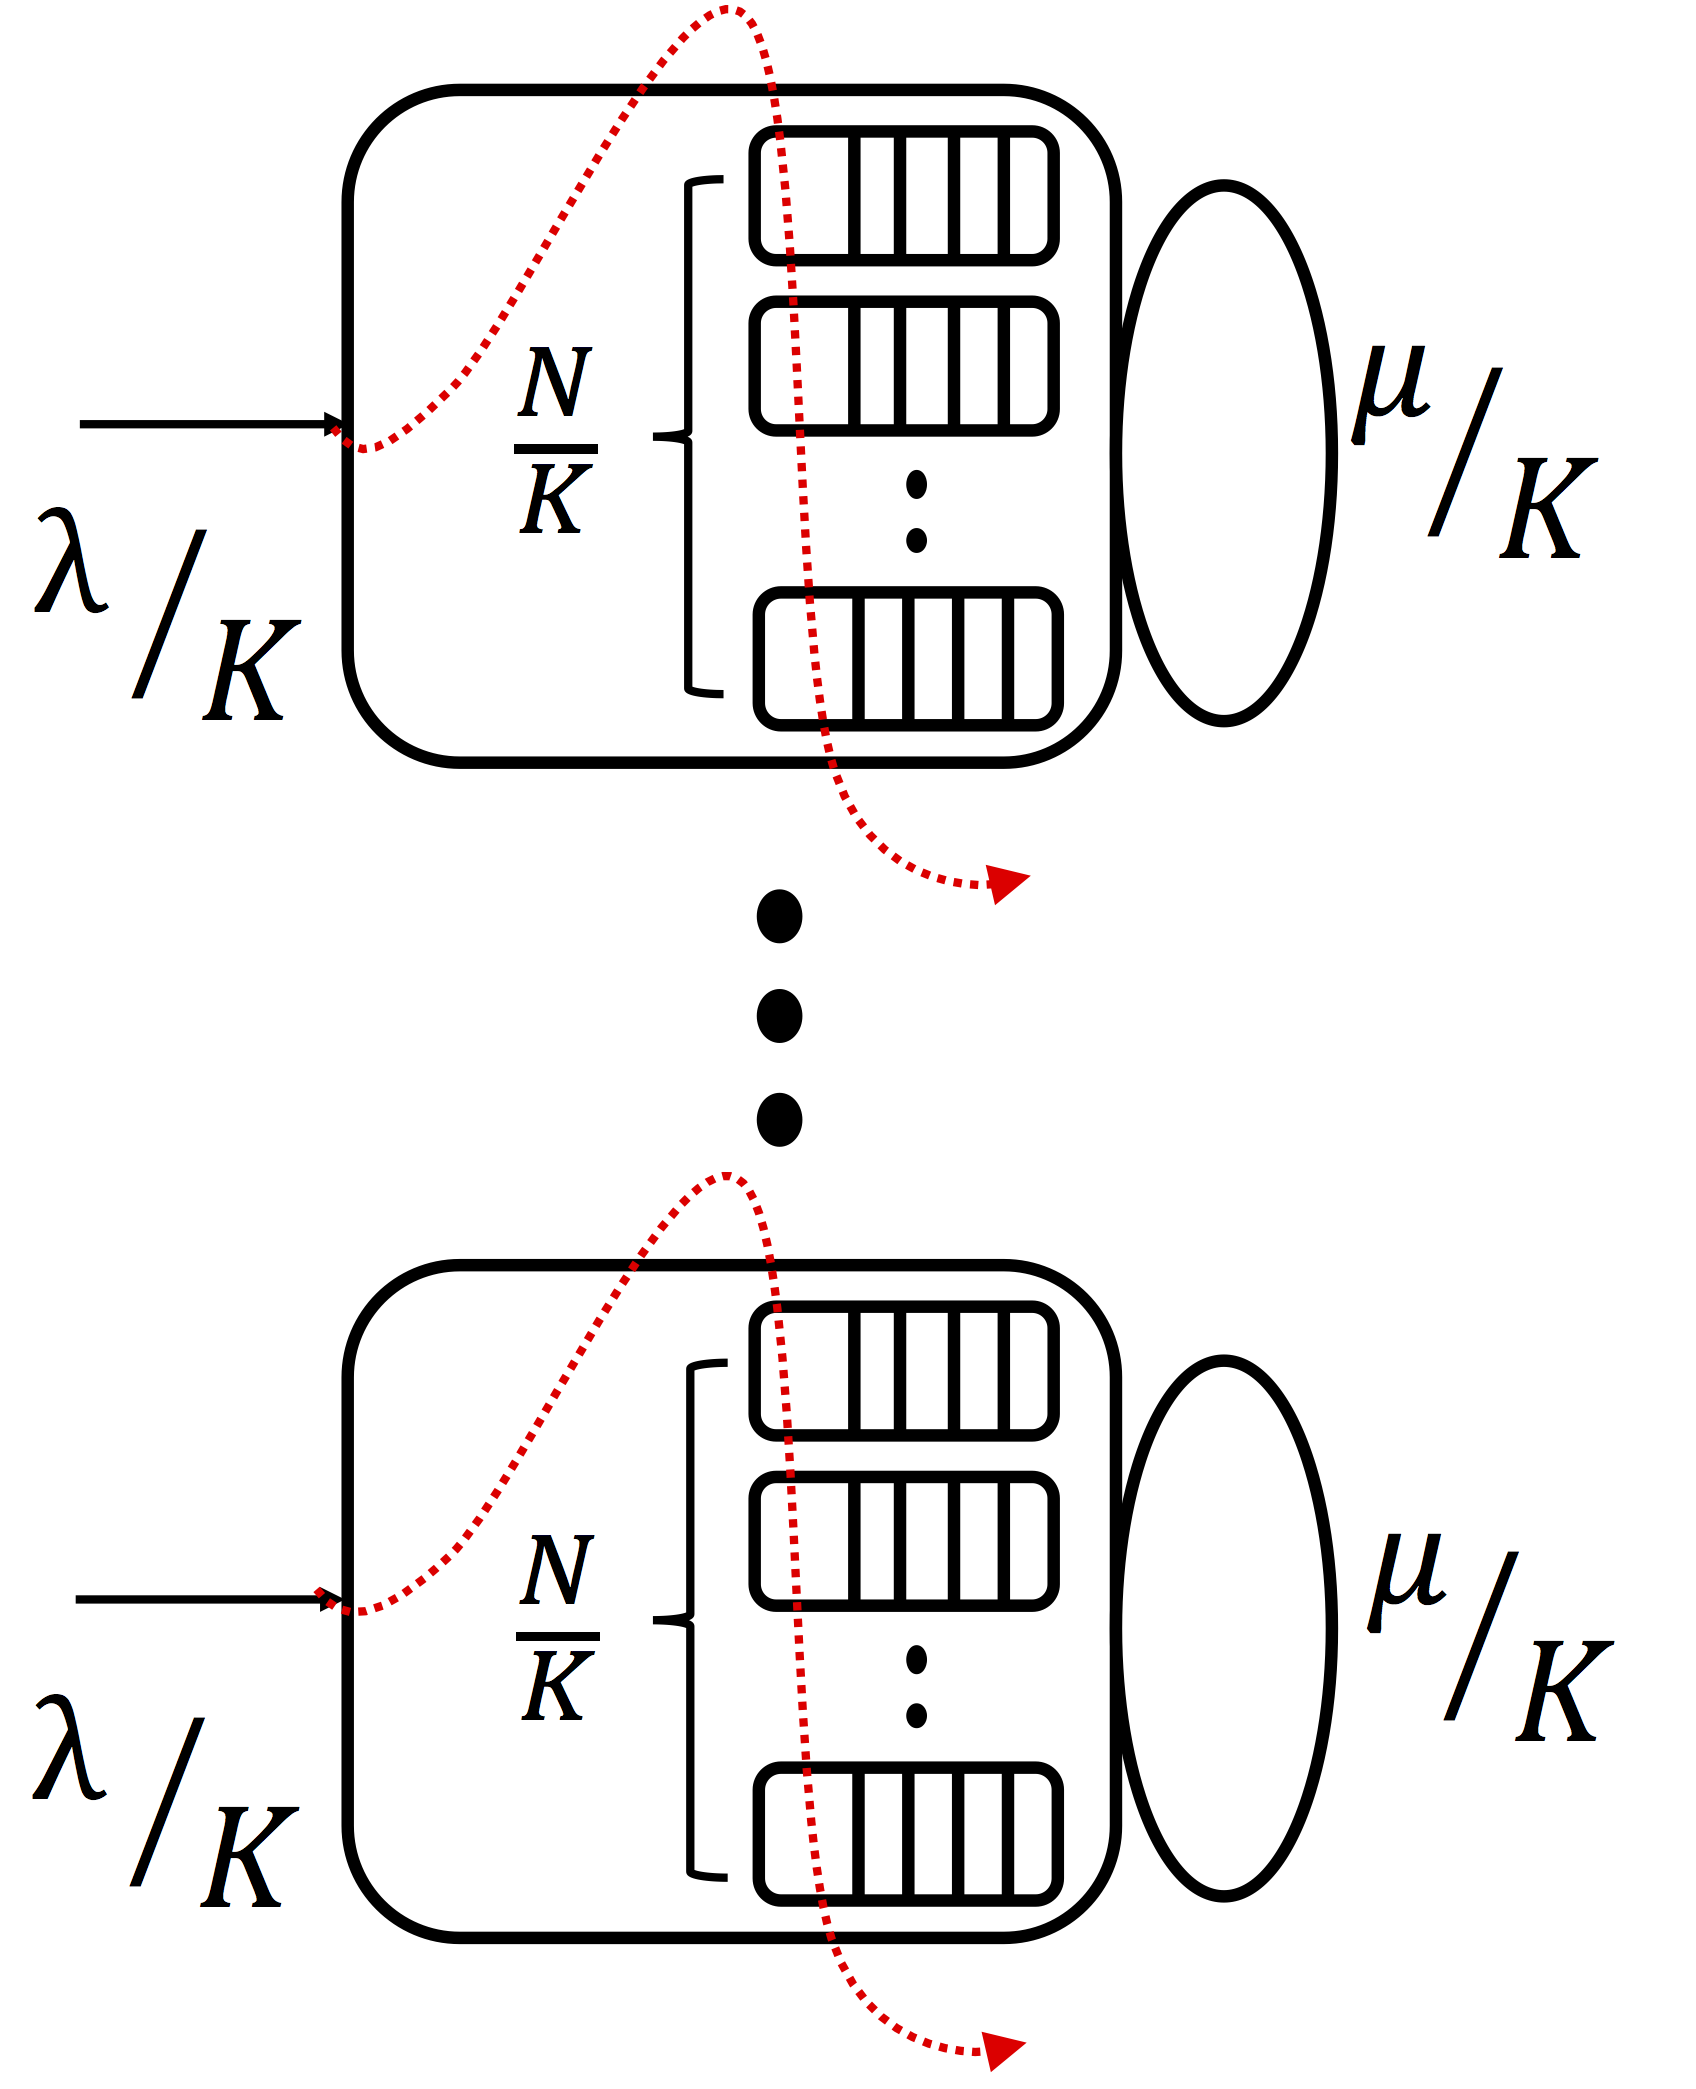
\includegraphics[width=0.8\textwidth]{Chapter3/Figures/esn}
		\caption{Independent servers}
		\label{fig:enn}
	\end{subfigure}
	\hfill
	\begin{subfigure}[b]{0.3\textwidth}
		\centering
		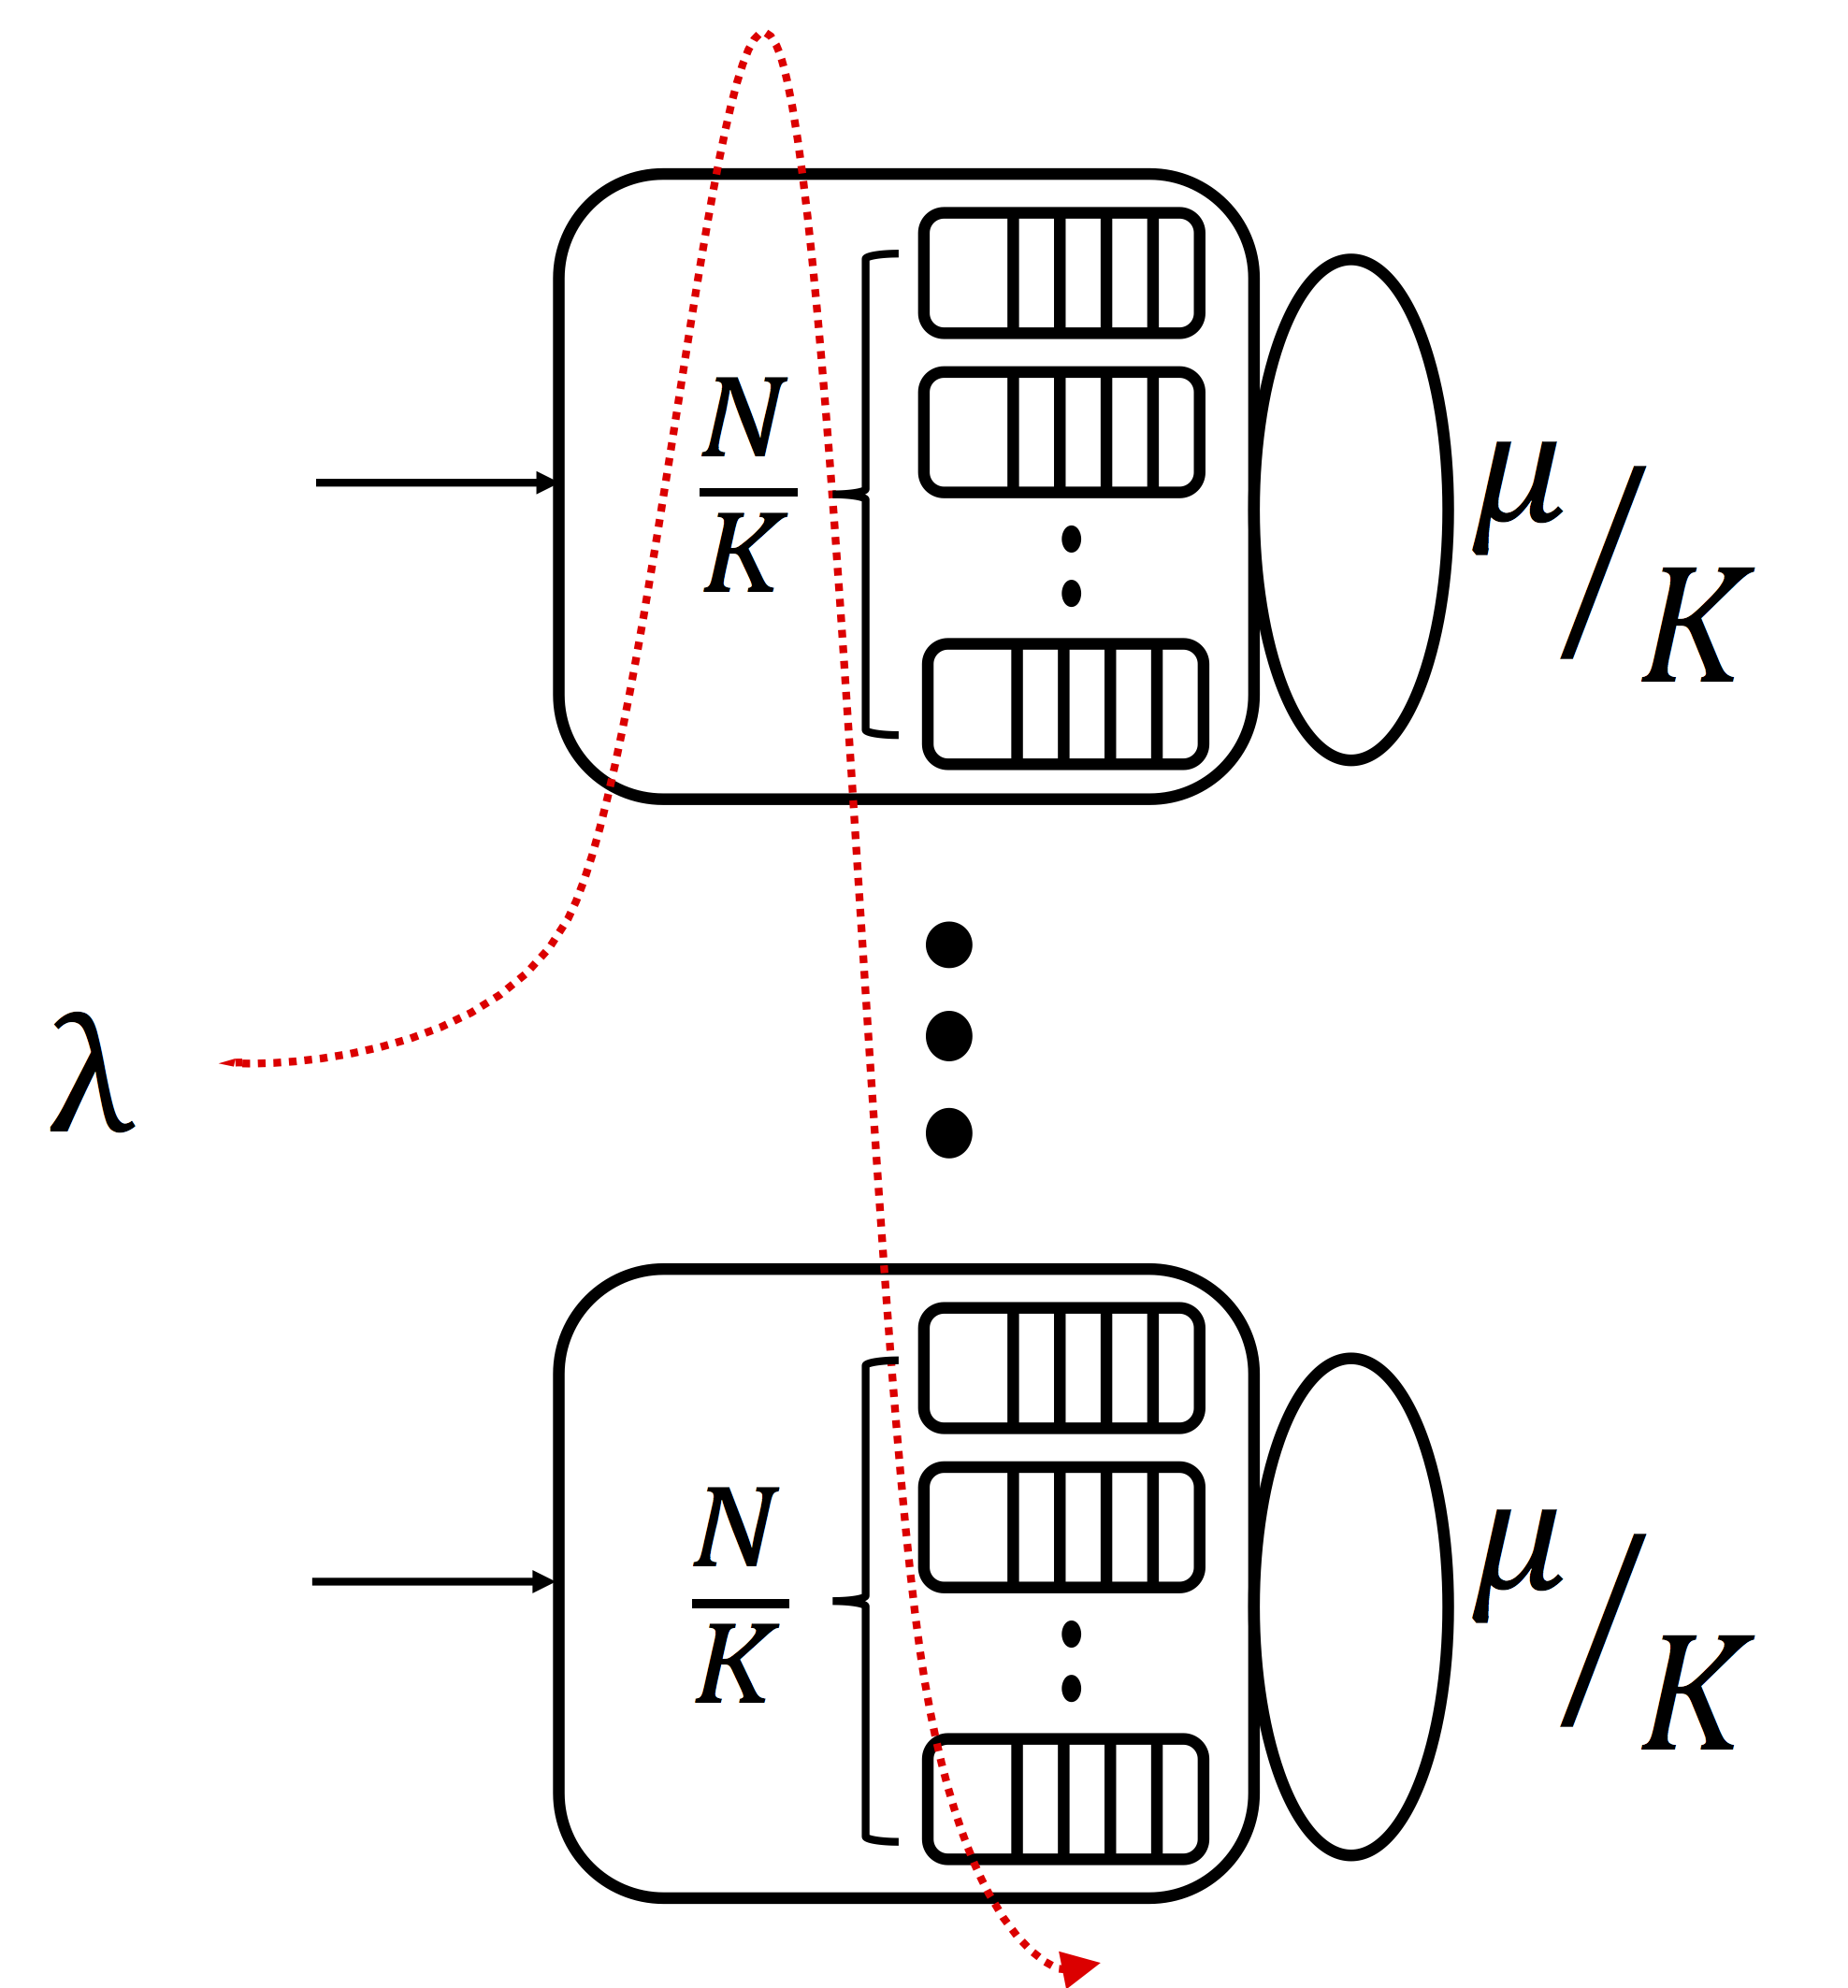
\includegraphics[width=0.9\textwidth]{Chapter3/Figures/sdmlfq}
		\caption{Spatial-diversity}
		\label{fig:sdmlfq}
	\end{subfigure}
	\caption{Three queuing system comparison.} %Red arrows indicate how queues are traversed during flow demotion. On each switch is reported the number of priorities it handles. Color scale is used to emphasize priority levels.}
	\label{fig:three-system-comparison}
\end{figure}

This is a general abstraction of the real system in a datacenter topology. At its heart, actually, a Leaf-and-Spine network with $K$ spines can be described with a scheme of $K$ parallel servers. These servers can be equivalently mapped to the \textit{up-send} interfaces that connects a ToR switch to all the spines, as well as to the \textit{down-send} interfaces that from different spines forward the traffic to a single ToR. Ingress and egress ports that connect end hosts to the datacenter network are ignored at this stage. This is in contrast with the data center abstraction of pFabric as a giant switch presented previously (Figure \ref{fig:pfabricdcn}), where the ingress and egress queues were the bottleneck links where to deploy best scheduling strategies. Also PIAS, optimizing its thresholds on the bottleneck link embraced a similar model. Somehow, differently from the state-of-the-art solutions that focus only on the bottleneck link assuming that with no oversubscription and ideal load balancing the network is able to sustain maximum throughput with negligible delays, the spatial-diversity approach shifts the attention on the queues inside the fabric itself. The integration with ingress and egress queues will be managed afterwards.\\
From now on and for the rest of this section, the interfaces abstracted in the simplified queuing model will be referred to as servers. The three systems are compared on the same conditions of total arrival rate $\lambda$, processing power $\mu$ and priority levels $N$, but with different partitioning of the same priority levels on a number $K$ of servers and, more importantly, with different demotion trajectories. Specifically, all systems use priority demotion first introduced by PIAS (\S \ref{sec:pias}). Red arrows indicate the trajectory across all available priority queues followed by the longest flow that experience the maximum number of demotions. \\
The first case (Fig. \ref{fig:switchone}) is to have a single high-capacity server that handles all priorities. This of course is the absolute best case where resources are fully concentrated, that doesn't exist in real systems and that provides the smallest delay. It would be equivalent to realize an entire data center interconnection network with a single device of astonishing bandwidth. The second case (Fig. \ref{fig:enn}) is the legacy way to handle priority demotion, where all servers are treated independently in parallel. Flows are evenly load balanced on the available servers and moved across priorities of the same server during their lifetime. In this case the number of demotion levels are limited to \small$\frac{N}{K}$\normalsize. Finally, the third case (Fig. \ref{fig:sdmlfq}) is the novel object under investigation, where all the flows are initially sent to the same server, then demoted on the $N$ globally available priority queues. In this case subsequent servers are configured to handle lower and lower priorities, thus part of the flows are re-routed as a consequence of the spatial-diversity. In the following, also the servers and the links may be labeled as "high priority" or "low priority" for brevity, meaning that they handle high priority traffic or low priority traffic, respectively. 

\subsection{Workloads}
The performances of the three systems are compared using two empirical flow size distributions that have been derived from production data centers (Figure \ref{fig:workloads}). Flow size distribution is shortly termed \emph{workload}. The first workload has been estimated instrumenting thousands of servers in a datacenter hosting a Web search \cite{dctcp} application, while the other refers to data mining tasks \cite{vl2}. 
\begin{figure}
	\centering
	\begin{subfigure}[b]{0.49\textwidth}
		\centering
		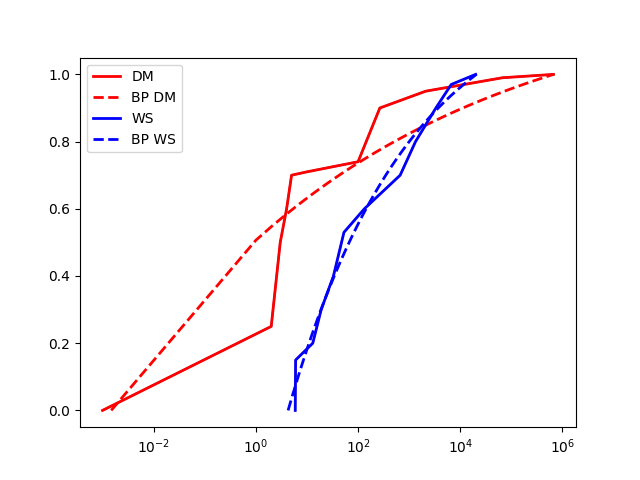
\includegraphics[width=\textwidth]{Chapter3/Figures/fits}
		\caption{CDF}
		\label{fig:cdfs}
	\end{subfigure}
   \hfill
   \begin{subfigure}[b]{0.49\textwidth}
   	\centering
   	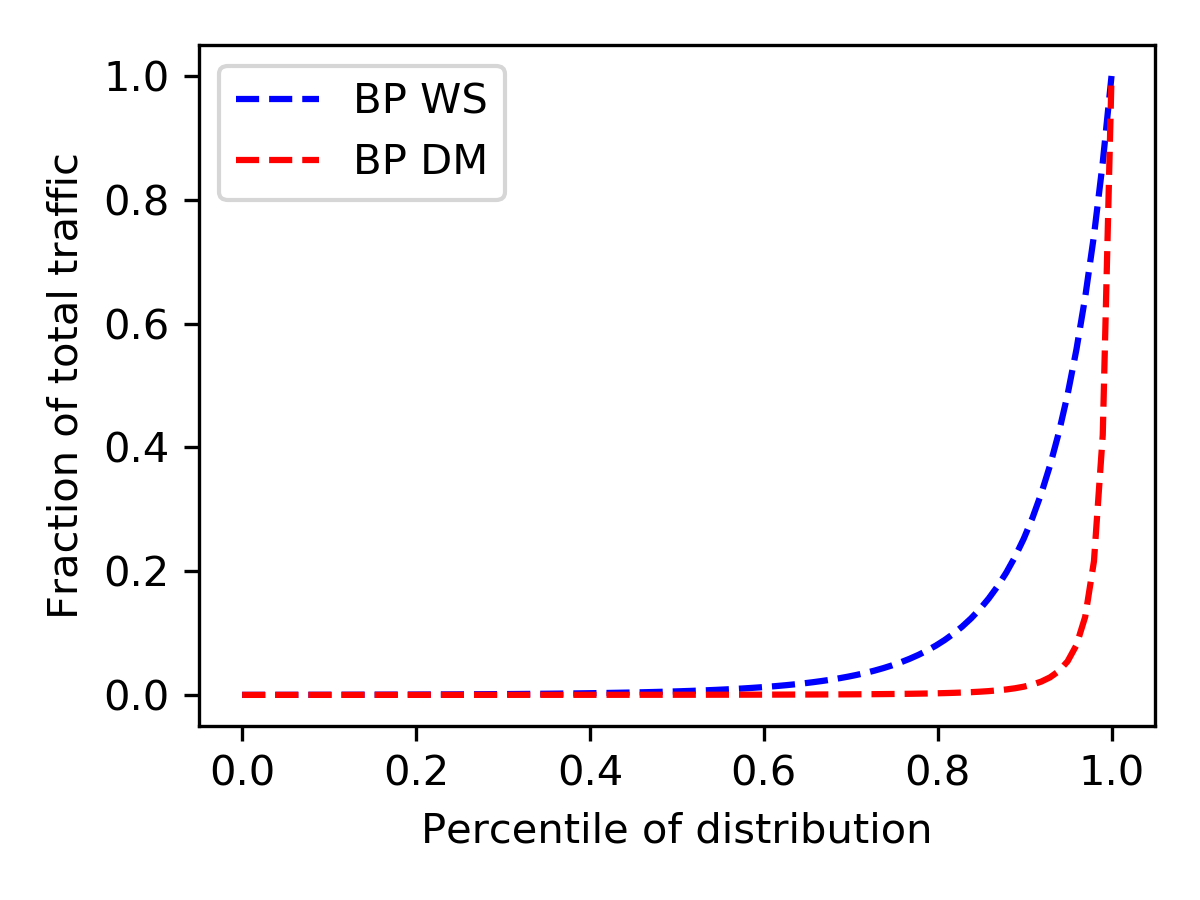
\includegraphics[width=\textwidth]{Chapter3/Figures/mwf}
   	\caption{MWF}
   	\label{fig:mwf}
   \end{subfigure}
	\caption{Workload properties}
	\label{fig:workloads}
\end{figure}
As expected, these distributions have a mix of short and long flows and both present the high-variability property typical of data center traffic (\S \ref{sec:traffic-properties}). Figure \ref{fig:cdfs} shows with solid lines the cumulative density function of the two empirical workloads, along with two dashed Bounded Pareto distributions, whose parameters have been fitted to the corresponding empirical points. The bounded Pareto distribution is a truncated version of the Pareto distribution over the finite support $[u,t]$ and it is well-suited to model heavy-tail characteristics. It has three parameter: the lower extreme of its support $u$, the upper extreme $t$ and the shape parameter $\alpha$ that controls the weight of its tail. The analytical expression of its cdf $F(x)$ in the interval $[u,t]$ is:
\begin{equation}
	F(x) = \dfrac{1-\Big(\dfrac{u}{x}\Big)^{\alpha}}{1-\Big(\dfrac{u}{t}\Big)^{\alpha}}, \qquad 0 \le \alpha \le 2
\end{equation}
This distribution has been chosen to be used in the analysis due to some graceful properties. First of all, it is relatively easy to control its variability by a proper tuning of its parameter $\alpha$. Values of $\alpha$ close to 2 accentuate the heavy-tail property, while smaller values of $\alpha$ tend to regularize a bit its behavior. Second, being definite on a limited support it can be adapted to any minimum and maximum flow size in the datacenter. Last, its mean and its variance  --- which depend on $\alpha$ --- are finite, thus the problem of finding the shape parameter for any fixed first and second moment can be smoothly treated numerically. Specifically, for the bounded Pareto, the mean and the variance have the following expression:
\begin{align*}
\mathbb{E}[X] &= \dfrac{\alpha}{(1-\alpha)(t^{\alpha}-u^{\alpha})} (u^{\alpha}t - t^{\alpha}u) \\ \\
\sigma_X^2 &= \dfrac{\alpha}{(2-\alpha)(t^{\alpha}-u^{\alpha})} (u^{\alpha}t^2 - t^{\alpha}u^2)
\end{align*}
The best fit to the empirical distributions has been obtained with a simple Maximum Likelihood Estimator (MLE). The resulting parameters are reported for both the workloads. Let $X$ be the flow size random variable as usual, and write in short notation \textit{BP}($u,t,\alpha$) the bounded Pareto. 
\begin{align*}
	X_{WS} \sim& \text{\textit{BP}}(3, \, 29000, \, 0.125)\\
	X_{DM} \sim& \text{\textit{BP}}(0.1, \, 100000, \,0.26)
\end{align*}
The measurement unit for the extremes of the support in this case is kilobytes. The fitting error is higher for the data mining workload than for the web search. For low percentiles this is difficult to avoid because a very crude sampling is provided. In fact, on a total of 11 empirical points, 4 of them are for values above the 90th percentile. Instead, for high percentiles a better fitting likely could be obtained by weighting more the tail of the distribution. However, since the simulations will be performed with the empirical traces, this point is neglected. \\
The rightmost plot (Fig. \ref{fig:mwf}) completes the picture by showing the Mass-Weighted Function $M_w(x)$ \cite{mwf}. This can be seen as the probability that a byte picked at random belongs to a flow below a given percentile and it is used to characterize the variability of a distribution. Its name comes from its definition, where job sizes are weighted by their probability mass:
\[
M_w(x) = \dfrac{\int_{0}^{x} x f(x) dx}{\mathbb{E}[X]}
\]
It holds:
\[
\int\nolimits_{0}^{x} x f(x) dx \le \mathbb{E}[X]
\]
In other words, it is just the average normalized traffic injected by flows shorter than $x$. The figure has on the abscissa the percentile rather than the corresponding job size, to allow the comparison between workloads with different supports on the same axis. If $y$ is a given percentile, it is evaluated $M_w(F^{-1}(y))$. \\
In summary, both distributions exhibit high variability. In the web search case the largest 4\% of flows carry half of the total traffic, the data mining is even more skewed: 70\% of the flows are less than 8 packets only, but almost the entire load is sustained by a ridiculous percentage of flows of about 100MB of size. This suggests that the more challenging distribution to schedule is the web search, consequently it is the one that will deserve most of the attention. In fact, recall that an ideal flow-agnostic LAS scheduler guarantees lower and lower delays as the variability of the distribution increases, both on average and at high percentiles (\S \ref{sec:las}). The theory is confirmed pretty straightforwardly by the simulation results presented next. Moreover, the web search distribution is also a lot easier to simulate, since the very long tails of the data mining workload require protracted time-consuming simulations before being precisely reproduced. Long flows occur sporadically, however they give the main contribution to generate a desired load on the system. 

\subsection{Optimal traffic load balancing}
In previous discussions, it was already realized that the spatial diversity framework introduces strong implications on how the load is distributed on the switching fabric, in particular on the bisection bandwidth. To clarify the concept let's come back to the abstract model considered so far and let's analyze the simpler example of spatial diversity, where only two M/M/1 servers are deployed in parallel, each of them with only a single priority queue. With this setup all flow demotions correspond to shifting a flow from one server to the other. Therefore, the assignment of the demotion threshold can be equivalently seen as a load balance problem. If the threshold is too small, flows are early rerouted on the low priority path and the capacity of the high priority link is essentially wasted. For the real data center implementation this would mean a 50\% throughput reduction of the switching fabric. On the other end, the traditional \textit{perfect} load balance which uniformly splits the traffic on available servers may correspond to a bad demotion threshold for the FCT minimization. Depending on the shape of the flow size distribution, latency constrained traffic would remain unnecessarily mixed with non-demanding latency flows. Certainly, the same issues arise the same augmenting the dimensionality of the topology and the priority queues. 
A careful tuning of load balance is a new trade-off that was nonexistent in the legacy MLFQ framework, where traffic was demoted to different priority queues but still in the same interface (i.e. link). If that is the case, a threshold setting that gives an unbalanced load allocation in the available priority queues affects only the delays but not the maximum throughput that the network can sustain. The introduction of spatial diversity adds a level of complexity to the system. 

Two related problems need to be solved: finding the set of thresholds that triggers a new flow route from one server to another and finding for each server a set of thresholds that mark the demotion boundaries among PQs. Let's denote them as \emph{load-balance thresholds} and \emph{sub-thresholds} respectively.
In section \ref{sec:complete-model} was presented an extension to the PIAS model that embeds spatial-diversity. This formulation would in principle address both problems. In fact, the optimal solution would never include load balance thresholds that overload some servers, because that would overkill the delays which the problem tries to minimize. At the same time, a unique formulation would choose a set of sub-thresholds targeted on the optimal load balance thresholds, providing a joint solution.  Despite being a clean analytical formulation, its complexity seems prohibitive. The basic model without spatial diversity yet was non-convex and presented products and ratios of unknowns (Sec. \ref{sec:pias-queueing-model}). Nonetheless, it is still tractable since the number of variables is typically bounded to the PQs available in commodity switches. Instead, in the complete model the number of variables scales with the product $K \times N$, where $K$ is usually a large number for large-scale data centers. An attempt for the web search workload and $K$$\times$$N$=16 was pursued with two well-known meta-heuristics solvers, specifically PSO \cite{pso,pso2} and Basin-Hoppin \cite{basinhoppin}. The time scale at which we could get a solution was at least days. Even finding an optimal solution once, it is not feasible to apply it to any real datacenter scenario where likely this solution must be computed repeatedly as statistics change.
To the purpose of investigating the spatial diversity framework, it has been preferred to handle the two problems individually. The approach that has been carried out is decoupled in two sequential steps.
\begin{enumerate}
	\item \textbf{Optimize load-balance thresholds.} First it is solved an optimization problem with the goal of finding the best load partitioning among $K$ servers. Servers are always assumed to have a single priority ($N$=1), because for the time being sub-thresholds are ignored. Subsequent servers are assigned increasing priorities, so that the number of demotions equals the number of servers and there are no duplicated priorities. At the end of this phase a set of $K$-1 load balance thresholds is delivered.
	\item \textbf{Greedy subthresholds}. The load-balance thresholds are provided as input of the second phase. They split the support of the flow size in $K$ disjoint intervals covering the whole support. The $i$-th interval contains the sizes of those flows that end their service in server of priority $i$. On each interval is computed a set of sub-thresholds with a greedy algorithm like ES-N or LS-N (Sec.\ref{sec:greedy-thresh}).  
	%Each of them truncates the original flow size distribution at a given percentile. 
\end{enumerate}
For the first phase turns out to be useful the stochastic queuing model of the legacy MLFQ system (Sec.\ref{sec:pias-queueing-model}-Fig.\ref{fig:pias_scheme}). After all, since each server is equipped with a single priority per port, the load balance problem can be abstracted with exactly the same model. The only exception is that the priority queues are physically distributed to different servers, instead of being part of the same interface. They are independent on each other and the strict priority scheduler is no more involved, as they work in parallel without coordination (Fig.\ref{fig:sdmlfq}). Practically, the only modification is to the queues capacities $\mu_i$. Remember that in the aforementioned model the strict priority order was described by attenuating the serving rates $\mu_i = \mu\prod_{i}(1-\rho_i)$ for increasing $i$. Because of servers work in parallel without scheduling, this expression is not needed anymore and the draining rates just coincide:
\[
\mu_i = \mu, \qquad i=1,..,K
\]
For the sake of simplicity, the $K$ parallel M/M/1 servers were implemented with service rate $\mu = \mathbb{E}[X]$. In this way the average load fed in the system 
\[
\rho = \frac{\lambda}{\mu}\;\mathbb{E}[X]
\]
is given only by the flow arrival intensity $\lambda$. \\
\begin{figure}
	\centering
	\begin{subfigure}{.5\textwidth}
		\centering
		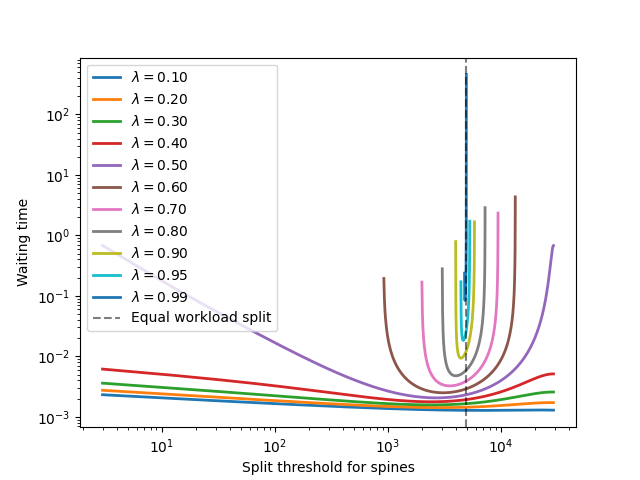
\includegraphics[width=.99\linewidth]{Chapter3/Figures/equal_workload_split_bpws}
		\caption{Optimal load balance threshold}
		\label{fig:cost-ws}
	\end{subfigure}%
	\begin{subfigure}{.5\textwidth}
		\centering
		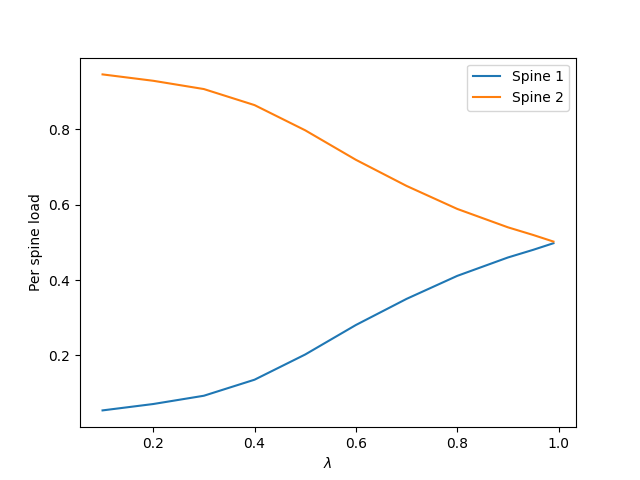
\includegraphics[width=.99\linewidth]{Chapter3/Figures/per_spine_load_bpdm}%TODO change fig with the one with crossing lines
		\caption{Load distribution per-server }
		\label{fig:perspineload-ws}
	\end{subfigure}
	\caption{Web search workload. Simple case of $K$=2.}
	\label{fig:lbthreshold-ws}
\end{figure}
\\
\begin{figure}
	\centering
	\begin{subfigure}{.5\textwidth}
		\centering
		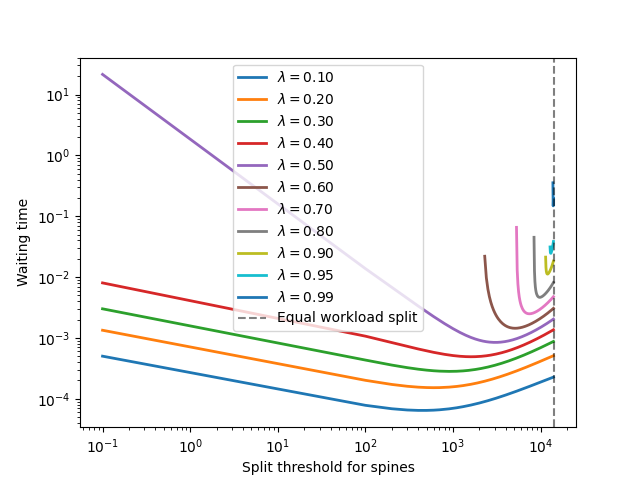
\includegraphics[width=.99\linewidth]{Chapter3/Figures/equal_workload_split_bpdm}
		\caption{Optimal load balance threshold}
		\label{fig:cost-dm}
	\end{subfigure}%
	\begin{subfigure}{.5\textwidth}
		\centering
		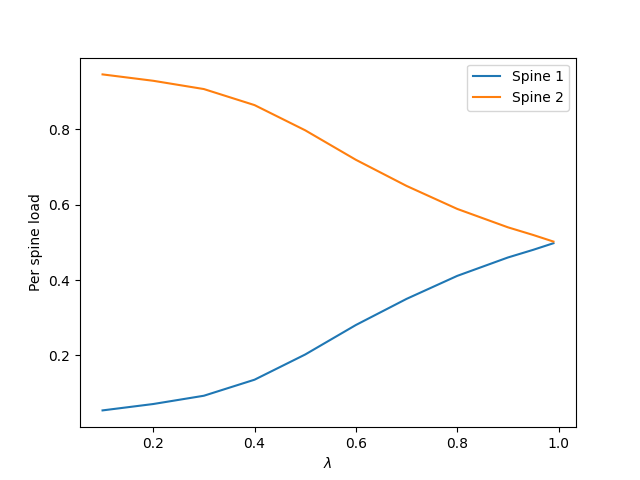
\includegraphics[width=.99\linewidth]{Chapter3/Figures/per_spine_load_bpdm}
		\caption{Load distribution per-server }
		\label{fig:perspineload-dm}
	\end{subfigure}
	\caption{Data mining workload. Simple case of $K$=2.}
	\label{fig:lbthreshold-dm}
\end{figure}
\subsubsection{Load balance on 2 parallel servers}
In the basic case of $K$=2 parallel servers, it is possible to plot the average sojourn time when varying the load balance threshold. Figures \ref{fig:cost-ws} and \ref{fig:cost-dm} show the aspect of the cost functions just described for the web search and the data mining workloads, respectively. All the axes are in log-scale and each curve represents a different normalized traffic $\lambda$. The vertical lines correspond the split that gives perfect load balance, apportioning half of the traffic on the high priority server and half on the low priority one. This split may be interchangeably referred to as \emph{perfect split} or \emph{proportionate split}. One phenomena is visible for both workloads, confirming previous intuitions. Imagine to connect the dots corresponding to the minima of the cost functions. The optimal load balance threshold does not coincide, broadly speaking, with the proportionate split threshold. Depending on the traffic level at which the system is operated and the workload, the optimal threshold triggers an earlier or later demotion with respect to the perfect split case. Equivalently, the jobs are distributed unfairly between the two servers (Figures \ref{fig:perspineload-ws}-\ref{fig:perspineload-dm}). For data mining, the imaginary line would be always in the leftmost side with respect to the proportionate split. That is, apart from loads close to saturation, the high priority server is kept as jobless as possible and the majority of work is sent to the low priority server. This result is coherent with the shape of the data mining workload, that presented huge variability. Plenty of short flows carrying few bytes are kept on a separated link from medium sized flows and a couple of long flows. This is not a surprise, since the problem formulation weighted more the average sojourn times of short flows. Slightly different trend is observed for web search. Moving from low to high values of $\lambda$, the optimal threshold is initially greater than the perfect split axis, then switches to its left and finally the two coincide. TODO Why??? For both cases, the objective function becomes much more extremely curled and steep around the perfect split axis when the load approaches the saturation value 1.  As already remarked, this is inevitable in order to fully exploit all the available capacity offered by the two parallel servers. At so high load any other traffic split would overload one of the two links and strongly deteriorate the average completion time of the flows going through it. Consistently, the cost function grows very rapidly in the neighborhood of the perfect split threshold value. \\
Finally, the two workloads have different sensitivities to the load balance threshold optimization. In particular, the web search achieves appreciable FCT gains starting from medium loads only ($\lambda > 0.5$) with (TODO provide some numbers), whereas at low loads there is no practical difference with the proportionate split. On the contrary, the data mining distribution gives theoretically a (TODO percentage) lower waiting time even for $\lambda$=0.1. This again reflects the extreme variability of the workload, that is comprised by a disproportionate number of short flows. The perfect split would keep a lot of mice flows mixed with low priority flows of bigger size for protracted service time. Instead, the optimal threshold reroute few flows but lot of traffic on the low priority server. In fact, for $\lambda$=0.1 the absolute value of the optimal threshold is an order of magnitude lower than the proportionate split threshold, however only a small fraction of flows fits into this gap. 

Summarizing, the above discussion confirms that the web search traffic is harder to cope with. This is the reason why in the following some results are shown exclusively for this workload.
\subsubsection{Validity of the model}

\subsubsection{Analysis of the model scalability}

\subsubsection{Finding sub-thresholds}

%TODO per spine load measured or plugged threshold in equation? 
\section{The service discipline: FIFO or PS?}

\subsection{Quantitative comparison}
FCT comparison: FIFO vs PS
\subsection{Flow synchronization}
Up to which point is spatial diversity meaningful? Flow synchronization problem. Burst arrivals. 
